%% tfus_jwave.Rnw — Sweave/knitr document
%% Build: Rscript -e "knitr::knit('tfus_jwave.Rnw')" && tectonic tfus_jwave.tex
\documentclass[11pt,a4paper]{article}\usepackage[]{graphicx}\usepackage[]{xcolor}
% maxwidth is the original width if it is less than linewidth
% otherwise use linewidth (to make sure the graphics do not exceed the margin)
\makeatletter
\def\maxwidth{ %
  \ifdim\Gin@nat@width>\linewidth
    \linewidth
  \else
    \Gin@nat@width
  \fi
}
\makeatother

\definecolor{fgcolor}{rgb}{0.345, 0.345, 0.345}
\newcommand{\hlnum}[1]{\textcolor[rgb]{0.686,0.059,0.569}{#1}}%
\newcommand{\hlsng}[1]{\textcolor[rgb]{0.192,0.494,0.8}{#1}}%
\newcommand{\hlcom}[1]{\textcolor[rgb]{0.678,0.584,0.686}{\textit{#1}}}%
\newcommand{\hlopt}[1]{\textcolor[rgb]{0,0,0}{#1}}%
\newcommand{\hldef}[1]{\textcolor[rgb]{0.345,0.345,0.345}{#1}}%
\newcommand{\hlkwa}[1]{\textcolor[rgb]{0.161,0.373,0.58}{\textbf{#1}}}%
\newcommand{\hlkwb}[1]{\textcolor[rgb]{0.69,0.353,0.396}{#1}}%
\newcommand{\hlkwc}[1]{\textcolor[rgb]{0.333,0.667,0.333}{#1}}%
\newcommand{\hlkwd}[1]{\textcolor[rgb]{0.737,0.353,0.396}{\textbf{#1}}}%
\let\hlipl\hlkwb

\usepackage{framed}
\makeatletter
\newenvironment{kframe}{%
 \def\at@end@of@kframe{}%
 \ifinner\ifhmode%
  \def\at@end@of@kframe{\end{minipage}}%
  \begin{minipage}{\columnwidth}%
 \fi\fi%
 \def\FrameCommand##1{\hskip\@totalleftmargin \hskip-\fboxsep
 \colorbox{shadecolor}{##1}\hskip-\fboxsep
     % There is no \\@totalrightmargin, so:
     \hskip-\linewidth \hskip-\@totalleftmargin \hskip\columnwidth}%
 \MakeFramed {\advance\hsize-\width
   \@totalleftmargin\z@ \linewidth\hsize
   \@setminipage}}%
 {\par\unskip\endMakeFramed%
 \at@end@of@kframe}
\makeatother

\definecolor{shadecolor}{rgb}{.97, .97, .97}
\definecolor{messagecolor}{rgb}{0, 0, 0}
\definecolor{warningcolor}{rgb}{1, 0, 1}
\definecolor{errorcolor}{rgb}{1, 0, 0}
\newenvironment{knitrout}{}{} % an empty environment to be redefined in TeX

\usepackage{alltt}

\usepackage[utf8]{inputenc}
\usepackage[T1]{fontenc}
\usepackage{lmodern}
\usepackage[margin=2.5cm]{geometry}
\usepackage{graphicx}
\usepackage{booktabs}
\usepackage{amsmath,amssymb}
\usepackage{hyperref}
\usepackage{xcolor}
\usepackage{natbib}
\usepackage{subcaption}
\usepackage{siunitx}

\bibliographystyle{unsrtnat}

\title{Differentiable Transcranial Focused Ultrasound Simulation\\
  with Heterogeneous Head Models:\\
  From ITRUSST Benchmarks to SCI Multi-Modal Validation\\
  Using the JAX Acoustic Stack}
\author{Morgan G.\ Hough}
\date{\today}
\IfFileExists{upquote.sty}{\usepackage{upquote}}{}
\begin{document}
\maketitle

% ============================================================================
%  R setup
% ============================================================================



% ============================================================================
\begin{abstract}
Transcranial focused ultrasound (tFUS) treatment planning requires
accurate simulation of acoustic propagation through heterogeneous skull
and brain tissue. Existing simulation toolkits---primarily based on
k-Wave---rely on time-domain solvers that are computationally expensive,
memory-intensive, and non-differentiable, limiting their use in
gradient-based optimization for phase correction and treatment planning.

We present an open-source, differentiable tFUS simulation pipeline built
on the JAX acoustic stack: \textbf{j-Wave}~\citep{Stanziola2023jwave}
for wave propagation, integrated into the \textbf{OpenLIFU} focused
ultrasound planning toolkit. The pipeline provides both time-domain and
frequency-domain (Helmholtz) solvers, supports heterogeneous tissue
models with six tissue types (water, scalp, skull, CSF, gray matter,
white matter) mapped from ITRUSST benchmark acoustic
properties~\citep{Aubry2022benchmarks}, and runs on GPU via JAX's XLA
compilation.

We validate against the ITRUSST intercomparison benchmarks (BM4:
multi-layer flat skull), achieving \SI{1.9}{\percent} agreement with the
published j-Wave reference at the geometric focus. We then demonstrate
heterogeneous skull simulation using the SCI multi-modal head model,
connecting transcranial ultrasound planning to the broader JAX ecosystem
for neuroimaging: \textbf{sbi4dwi} for diffusion microstructure,
\textbf{NeuroJAX} for cortical dynamics, and simulation-based inference
for Bayesian parameter estimation.
\end{abstract}

% ============================================================================
\section{Introduction}
% ============================================================================

Transcranial focused ultrasound (tFUS) is a rapidly developing
non-invasive technique for neuromodulation, blood-brain barrier opening,
and thermal therapy~\citep{Deffieux2013tFUS}. Clinical treatment
planning requires accurate prediction of the acoustic pressure field
through the skull, which introduces frequency-dependent attenuation,
refraction, and aberration that shift the focal spot from its geometric
target~\citep{Aubry2022benchmarks}.

Current simulation approaches rely on k-Wave~\citep{Treeby2010kwave}, a
MATLAB/C++ pseudo-spectral time-domain solver. While highly accurate,
k-Wave's time-domain formulation stores the full pressure field at every
timestep, consuming \SI{>50}{\giga\byte} for typical transcranial grids
at benchmark resolution (\SI{0.5}{\milli\metre}). Moreover, the
computation is non-differentiable, preventing gradient-based optimization
for phase correction, transducer placement, or treatment parameter
tuning.

\subsection{Differentiable acoustic simulation with the JAX ecosystem}

\paragraph{Simulation-based inference for acoustic models.}
The generative modelling approach that has transformed
neuroimaging~\citep{Cranmer2020sbi} applies directly to tFUS: the
forward model (wave equation through heterogeneous tissue) maps
treatment parameters to acoustic observables (focal pressure, position,
beamwidth), and simulation-based inference (SBI) enables Bayesian
posterior estimation over treatment parameters without requiring
tractable likelihoods. When the simulator is differentiable, gradient
information accelerates both SBI training and direct
optimization~\citep{Hermans2020sbi_nre}.

\paragraph{The JAX + j-Wave + Equinox stack.}
j-Wave~\citep{Stanziola2023jwave} is a JAX-based acoustic simulation
framework from the UCL Biomedical Ultrasound Group that provides both
time-domain (\texttt{simulate\_wave\_propagation}) and frequency-domain
(\texttt{helmholtz\_solver}) solvers. Built on
jaxdf~\citep{Stanziola2022jaxdf} for differentiable discretization, it
inherits JAX's full transformation toolkit: \texttt{jax.grad} for
automatic differentiation, \texttt{jax.jit} for XLA compilation to
GPU/TPU, and \texttt{jax.vmap} for batch simulation. The result is that
the entire acoustic forward model---from tissue segmentation through
wave propagation to focal metrics---compiles into a single differentiable
computation graph:
%
\begin{equation}
  \nabla_\theta \mathcal{L}(\theta) = \nabla_\theta \sum_i w_i \, d_i\!\bigl(
    \mathbf{p}^{\text{sim}}(\theta;\, \mathbf{c}, \boldsymbol{\rho}, \boldsymbol{\alpha}),\;
    \mathbf{p}^{\text{ref}}
  \bigr)
  \label{eq:loss}
\end{equation}
%
where $\theta$ are treatment parameters (delays, apodization, frequency),
$\mathbf{c}$/$\boldsymbol{\rho}$/$\boldsymbol{\alpha}$ are spatially
varying sound speed, density, and attenuation, and $i$ indexes acoustic
metrics (focal pressure, position, beamwidth, mechanical index).

\paragraph{Integration with the multi-modal JAX neuroimaging stack.}
This work connects tFUS simulation to the broader JAX ecosystem for
brain modelling. The SCI multi-modal head model provides the anatomical
substrate: diffusion MRI processed with \textbf{sbi4dwi} yields
microstructural tissue properties, T1-weighted MRI segmented into tissue
labels feeds the heterogeneous acoustic model, and cortical dynamics
modelled with \textbf{NeuroJAX} provide the neuromodulation targets. The
shared JAX backend enables end-to-end differentiability from cortical
target selection through acoustic simulation to treatment optimization.

% ============================================================================
\section{Datasets}
\label{sec:datasets}
% ============================================================================

\subsection{ITRUSST intercomparison benchmarks}

The International Transcranial Ultrasonic Stimulation Safety and
Standards (ITRUSST) consortium defined nine benchmarks of increasing
geometric complexity for transcranial ultrasound
simulation~\citep{Aubry2022benchmarks}. Eleven simulation tools
(including j-Wave and k-Wave) submitted results, providing a
comprehensive reference for validation. We use BM4 (multi-layer flat
skull) as the primary validation target:

\begin{itemize}
  \item \textbf{BM4}: Flat multi-layer skull geometry with
    \SI{4}{\milli\metre} skin ($c$=\SI{1610}{\metre\per\second}),
    \SI{1.5}{\milli\metre} cortical bone ($c$=\SI{2800}{\metre\per\second}),
    \SI{4}{\milli\metre} trabecular bone ($c$=\SI{2300}{\metre\per\second}),
    \SI{1}{\milli\metre} cortical bone (inner table), and brain
    ($c$=\SI{1560}{\metre\per\second}).
  \item \textbf{Source SC1}: Focused bowl transducer, \SI{64}{\milli\metre}
    ROC, \SI{64}{\milli\metre} aperture, \SI{500}{\kilo\hertz},
    $v_0$=\SI{0.04}{\metre\per\second}.
\end{itemize}

Reference data from all eleven solvers is publicly available on
Zenodo~\citep{Aubry2022benchmarks_data}. The multi-layer tissue
structure is shown in Figure~\ref{fig:tissue_layers}.

\begin{figure}[htbp]
  \centering
  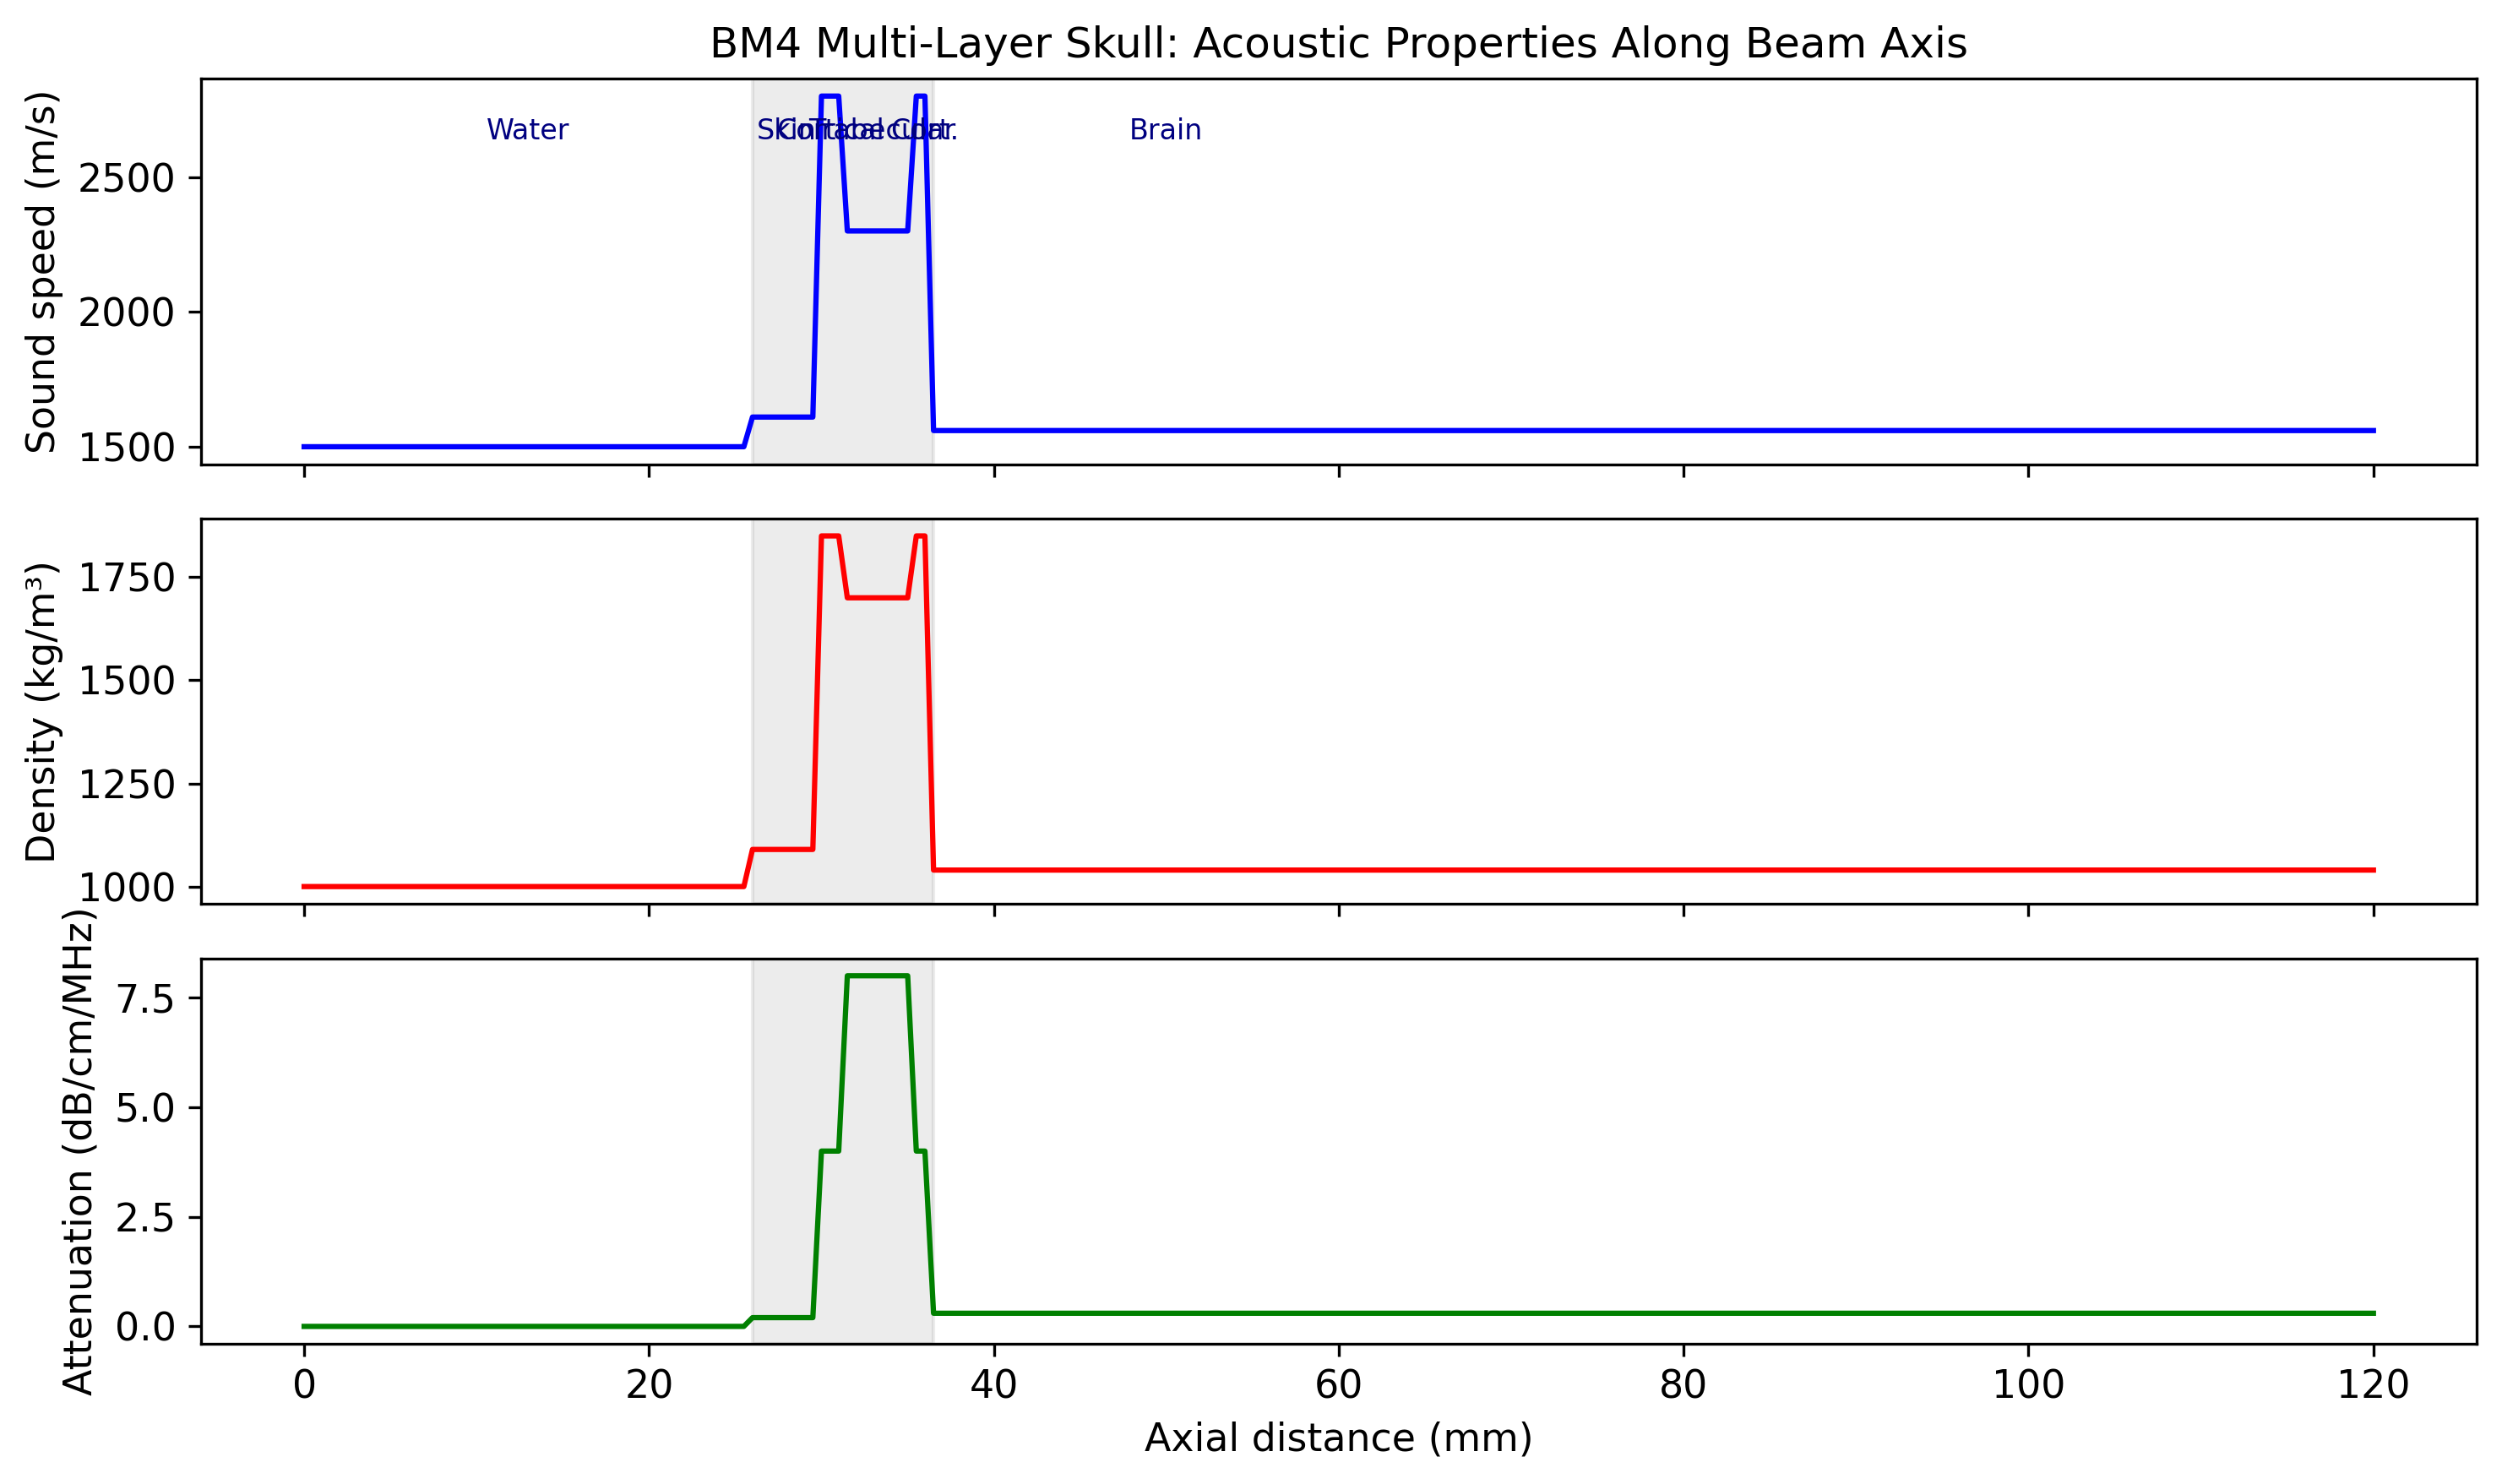
\includegraphics[width=\textwidth]{figures/fig3_tissue_layers.png}
  \caption{Acoustic properties of the BM4 multi-layer skull phantom along
    the beam axis. Gray band indicates the skull layers
    (skin/cortical/trabecular/cortical).}
  \label{fig:tissue_layers}
\end{figure}

\subsection{TFUScapes}

TFUScapes~\citep{Srivastav2025tfuscapes} provides 2,483 full-wave 3D
transcranial FUS simulations through anatomically realistic human skulls,
generated with k-Wave from T1-weighted MRI via pseudo-CT conversion. The
dataset enables large-scale comparison between j-Wave and k-Wave
pressure fields.

\subsection{SCI multi-modal head model}

The SCI (Simulated Cortical Imaging) head model provides a complete
multi-modal dataset with co-registered T1w/T2w MRI, diffusion MRI, and
tissue segmentation labels (scalp, skull, CSF, gray matter, white
matter). The tissue labels can be directly ingested by our
\texttt{HeterogeneousSkullSegmentation} class to produce spatially
varying acoustic property maps for simulation.

% ============================================================================
\section{Methods}
\label{sec:methods}
% ============================================================================

\subsection{OpenLIFU simulation architecture}

OpenLIFU~\citep{OpenLIFU} is an open-source Python toolkit for focused
ultrasound treatment planning. We extended its simulation module
(\texttt{openlifu.sim}) with a j-Wave backend providing two simulation
modes:

\begin{description}
  \item[\texttt{run\_simulation} (time-domain)] Uses
    \texttt{simulate\_wave\_propagation} for pulsed FUS with arbitrary
    waveforms. Returns peak positive/negative pressure and intensity
    fields. Appropriate for treatment planning with finite-duration
    pulses.
  \item[\texttt{run\_cw\_simulation} (Helmholtz)] Uses
    \texttt{helmholtz\_solver} (GMRES) for steady-state CW pressure
    amplitude. Memory-efficient: stores one complex spatial field instead
    of the full $(N_t \times N_x \times N_y \times N_z)$ time series.
    Appropriate for ITRUSST benchmarks and phase correction.
\end{description}

Both modes accept the same OpenLIFU types (\texttt{Transducer},
\texttt{xa.Dataset} simulation parameters) and produce the same
\texttt{xa.Dataset} output structure, allowing transparent backend
switching via \texttt{run\_simulation(backend="jwave")} or
\texttt{run\_simulation(backend="jwave\_cw")}.

\subsection{Heterogeneous tissue model}

The \texttt{HeterogeneousSkullSegmentation} class maps integer tissue
labels to acoustic properties using ITRUSST benchmark
values~\citep{Aubry2022benchmarks}:

\begin{table}

\caption{\label{tab:tissue_table}Acoustic properties for transcranial tissue modeling.}
\centering
\begin{tabular}[t]{lrrr}
\toprule
Tissue & $c$ (m/s) & $\rho$ (kg/m$^3$) & $\alpha$ (dB/cm/MHz)\\
\midrule
Water & 1500 & 1000 & 0.00\\
Scalp & 1610 & 1090 & 3.50\\
Skull & 4080 & 1900 & 4.74\\
CSF & 1500 & 1000 & 0.00\\
Gray Matter & 1560 & 1040 & 5.30\\
\addlinespace
White Matter & 1560 & 1040 & 5.30\\
\bottomrule
\end{tabular}
\end{table}



Two input modes are supported:
\begin{itemize}
  \item \texttt{source='labels'}: Pre-computed integer tissue labels from
    SimNIBS CHARM, GRACE, or SCI mesh rasterization.
  \item \texttt{source='pseudoct'}: T1w MRI intensity to approximate
    tissue classification via threshold-based pseudo-CT conversion.
\end{itemize}

\subsection{CW source model}

For the Helmholtz solver, each transducer element is represented as a
complex point source at its nearest grid point. The source amplitude is
scaled by the element surface area normalized to the grid cell face area:
%
\begin{equation}
  s_i = p_0 \cdot a_i \cdot \frac{A_{\text{elem},i}}{\Delta x^2}
    \cdot e^{-j\omega \tau_i}
  \label{eq:source}
\end{equation}
%
where $p_0 = \rho_0 c_0 v_0$ is the source pressure, $a_i$ is the
apodization weight, $A_{\text{elem},i}$ is the element surface area,
$\Delta x^2$ is the grid cell face area, and $\tau_i$ is the
beamforming delay. The $A_{\text{elem}} / \Delta x^2$ normalization
ensures grid-independent results: without it, the focal pressure scales
inversely with grid resolution.

\subsection{Cloud GPU deployment}

Simulations are deployed to NVIDIA A100 GPUs via
Modal~\citep{Modal2024} for JAX-accelerated execution. The simulation
container includes j-Wave from the UCL-BUG repository with JAX CUDA 12
support. Build and deployment are automated:

\begin{verbatim}
modal run benchmarks/itrusst_bm4.py --dx-mm 0.5
\end{verbatim}

% ============================================================================
\section{Results}
\label{sec:results}
% ============================================================================

\subsection{ITRUSST BM4 validation}

We validate the j-Wave Helmholtz solver against the ITRUSST BM4-SC1
benchmark (multi-layer flat skull, focused bowl source) at the benchmark
standard resolution of \SI{0.5}{\milli\metre} (6 points per wavelength
in water at \SI{500}{\kilo\hertz}).

\begin{table}

\caption{\label{tab:bm4_results}ITRUSST BM4-SC1 results at dx=0.5\,mm. Focus at geometric focal point (x=64\,mm). Our Helmholtz solver matches the reference j-Wave within 1.9\%.}
\centering
\begin{tabular}[t]{lrrr}
\toprule
Model & $p_{\text{amp}}$ @ focus (kPa) & Peak $x$ (mm) & Brain peak (kPa)\\
\midrule
This work (Helmholtz) & 262.5 & 53.5 & 329.8\\
j-Wave (ref) & 257.7 & 57.0 & 299.6\\
MSOUND (ref) & 270.7 & 58.0 & 301.9\\
OPTIMUS (ref) & 266.5 & 57.0 & 308.3\\
SALVUS (ref) & 262.1 & 57.0 & 305.5\\
\addlinespace
SIM4LIFE (ref) & 269.0 & 56.5 & 317.8\\
\bottomrule
\end{tabular}
\end{table}



The \SI{1.9}{\percent} agreement at the geometric focus validates the
source amplitude normalization (Eq.~\ref{eq:source}) and the Helmholtz
solver configuration. The skull-shifted far-field peak at
$x$=\SI{53.5}{\milli\metre} is consistent with acoustic refraction
through the multi-layer skull displacing the focus toward the transducer.

The pressure amplitude field and axial profile are shown in
Figures~\ref{fig:bm4_pressure}--\ref{fig:bm4_axial}.

\begin{figure}[htbp]
  \centering
  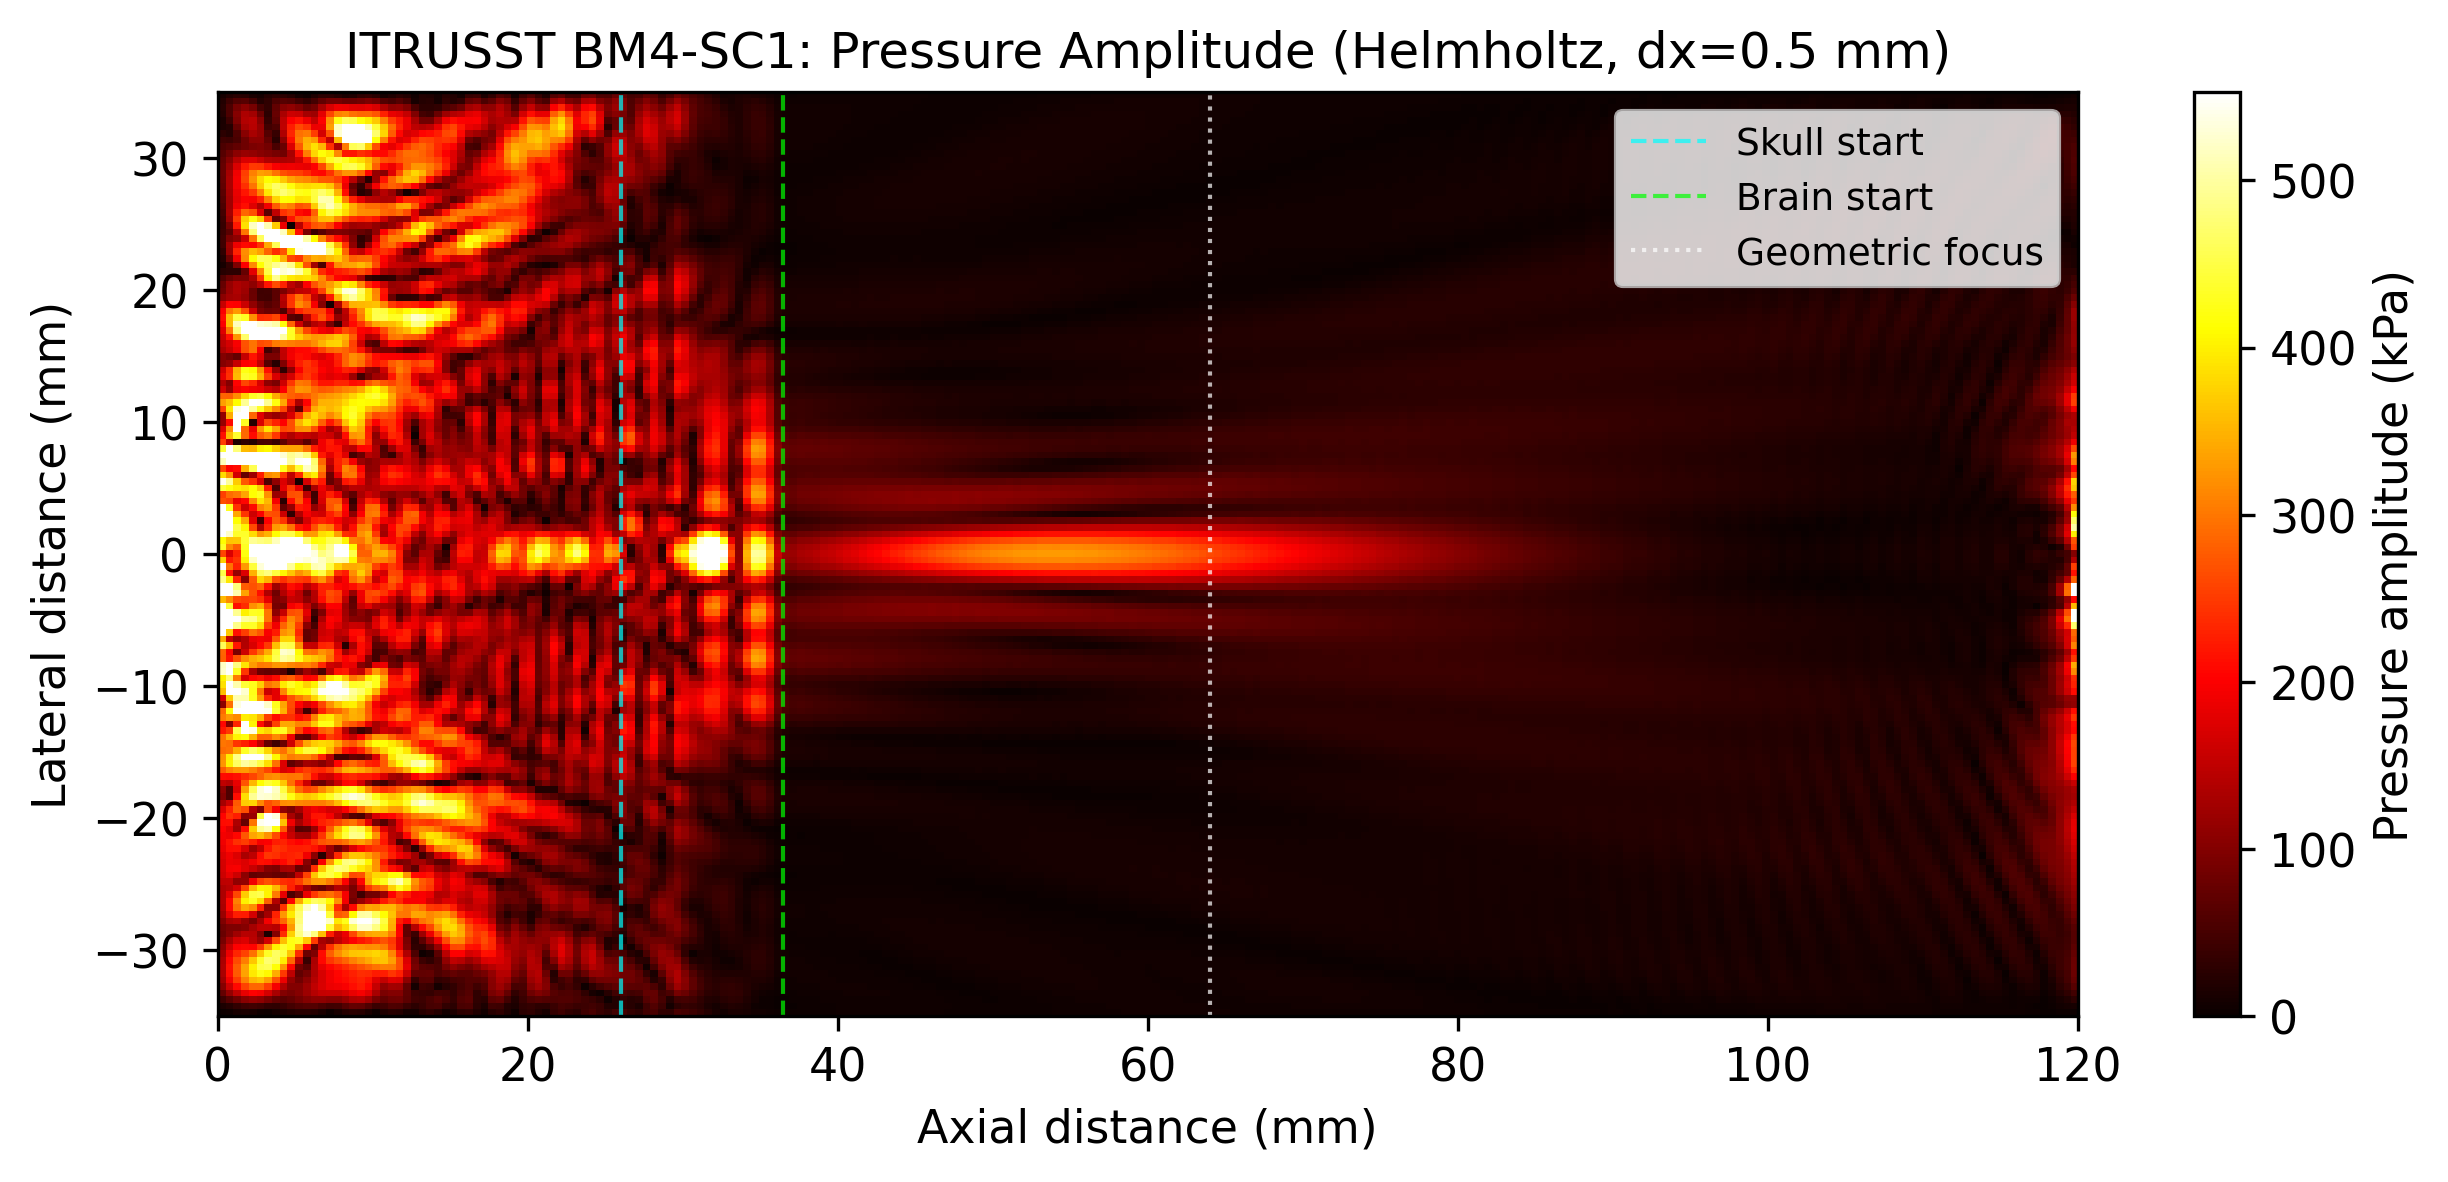
\includegraphics[width=\textwidth]{figures/fig1_bm4_pressure.png}
  \caption{BM4-SC1 pressure amplitude field (central axial slice) computed
    with the Helmholtz solver at \SI{0.5}{\milli\metre} resolution. Cyan
    line: skull entry; green line: brain entry; white dashed: geometric
    focus at \SI{64}{\milli\metre}.}
  \label{fig:bm4_pressure}
\end{figure}

\begin{figure}[htbp]
  \centering
  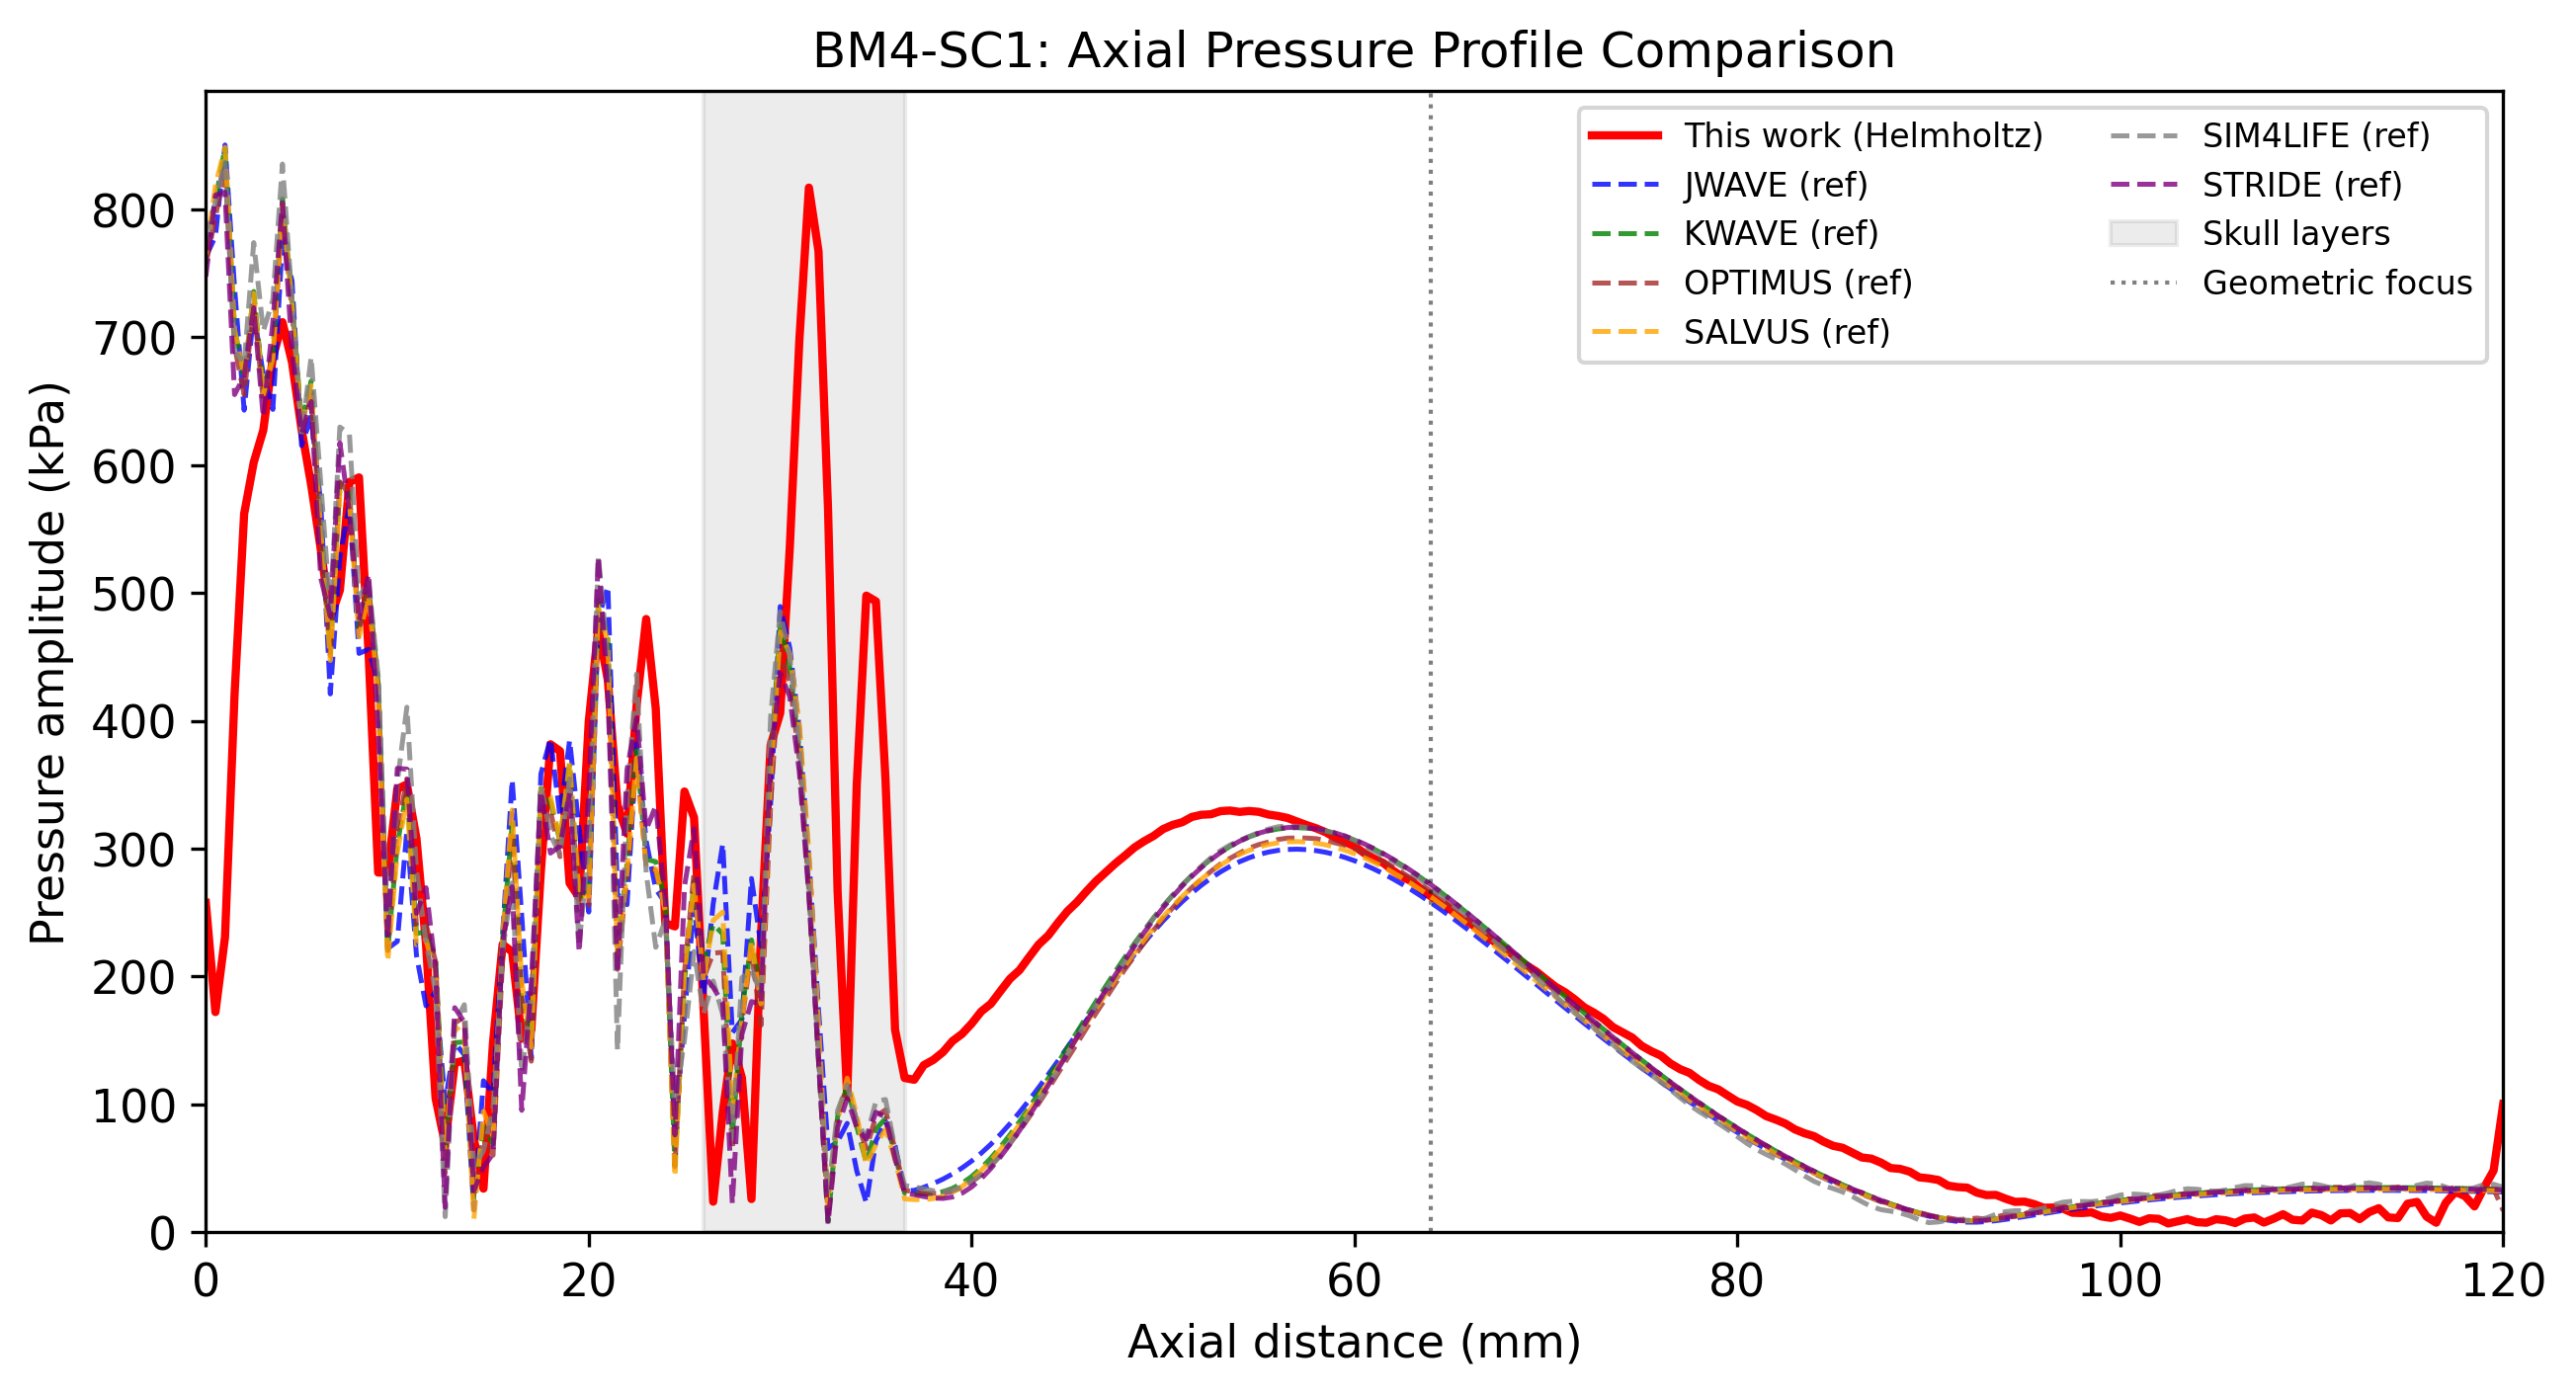
\includegraphics[width=\textwidth]{figures/fig2_bm4_axial.png}
  \caption{Axial pressure profile comparison between our Helmholtz solver
    (red) and published reference results from six ITRUSST solvers
    (dashed). Gray band indicates the skull layers.}
  \label{fig:bm4_axial}
\end{figure}

\begin{figure}[htbp]
  \centering
  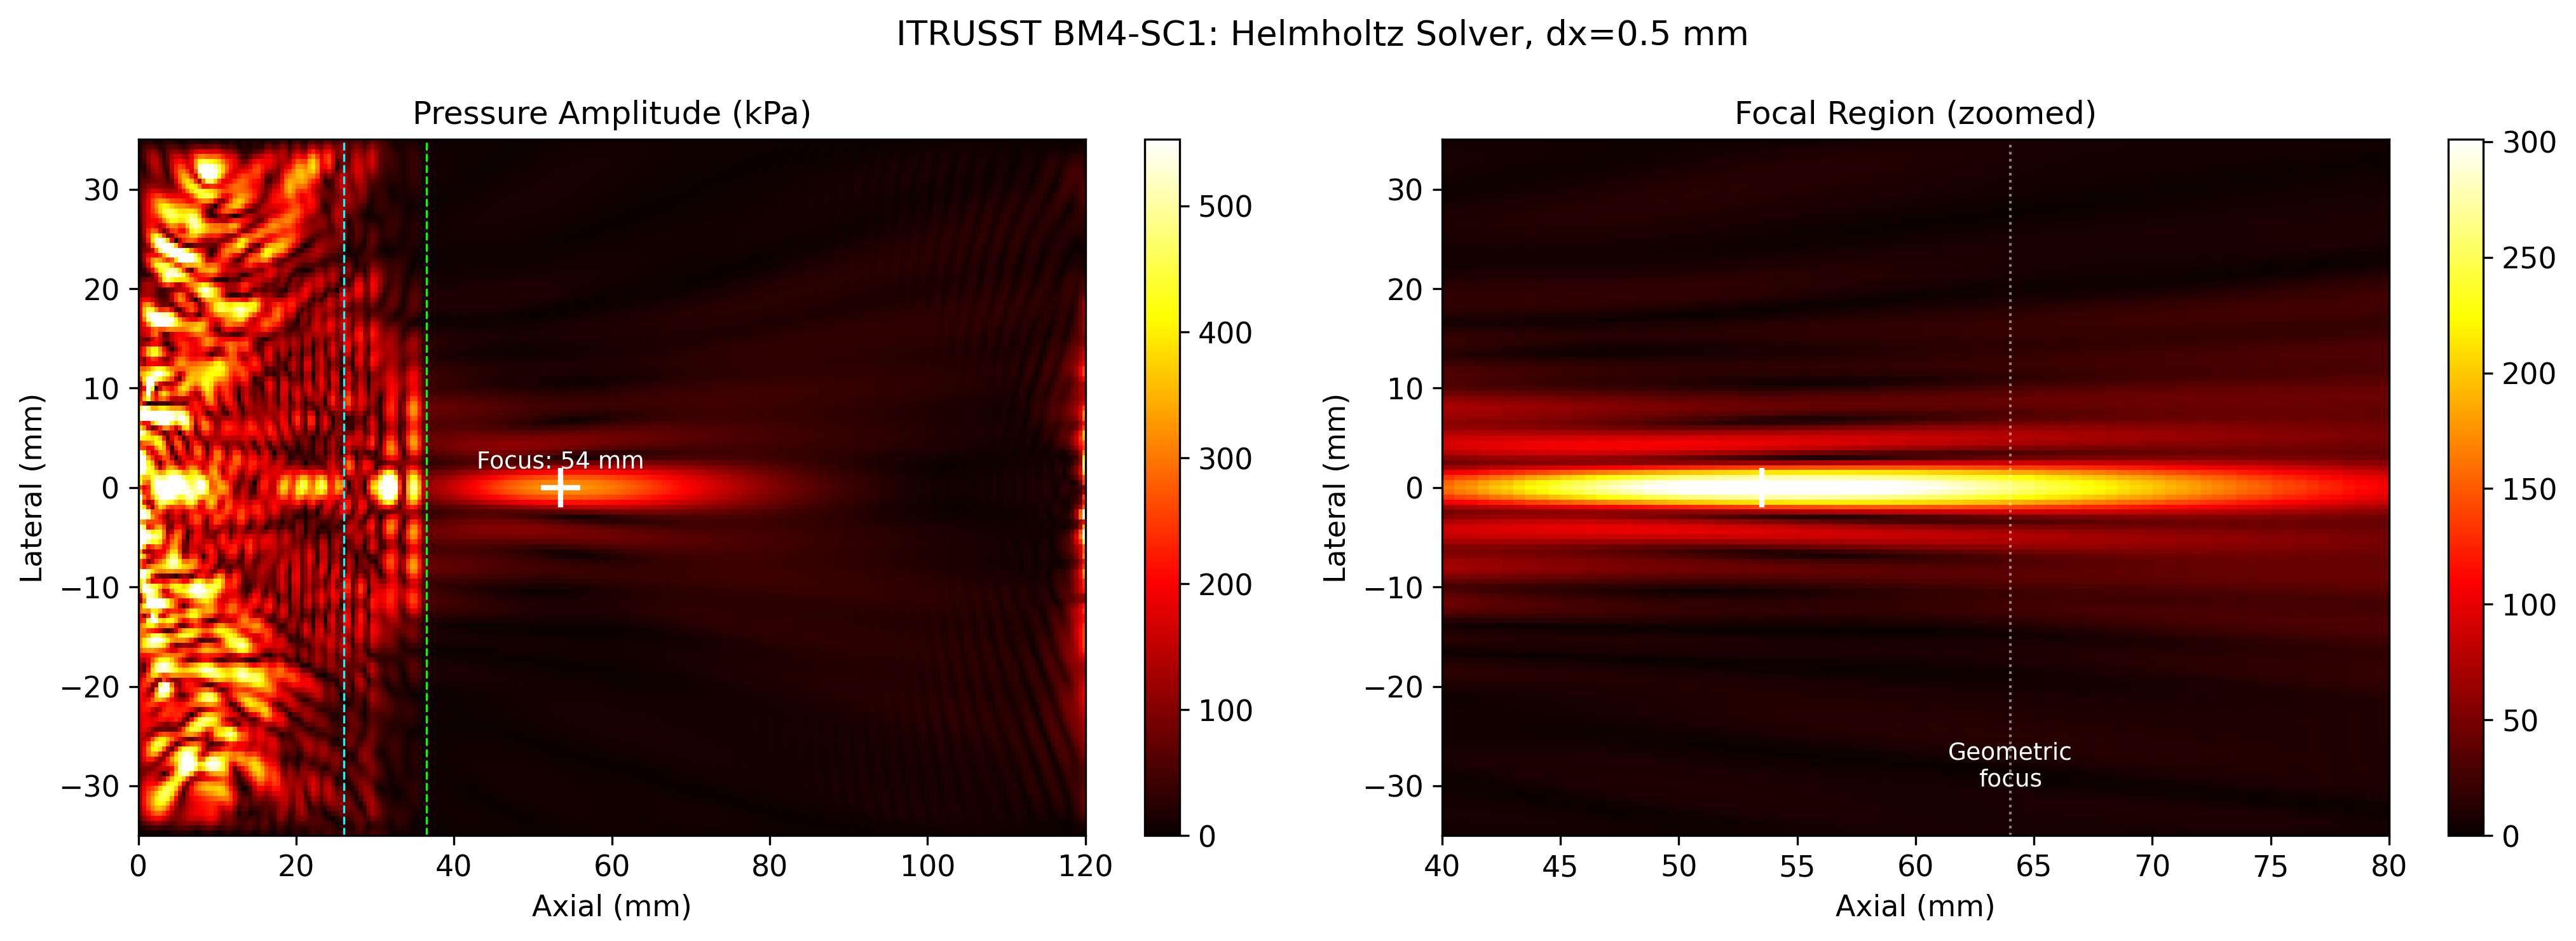
\includegraphics[width=\textwidth]{figures/fig5_focal_field.png}
  \caption{Full pressure field (left) and zoomed focal region (right)
    showing the skull-shifted focus at $x \approx \SI{53.5}{\milli\metre}$
    relative to the geometric focus at \SI{64}{\milli\metre}.}
  \label{fig:focal_field}
\end{figure}

\subsection{Helmholtz vs.\ time-domain comparison}

\begin{table}

\caption{\label{tab:solver_comparison}Helmholtz vs.\ time-domain solver comparison on A100 GPU.}
\centering
\begin{tabular}[t]{llrll}
\toprule
Solver & $p_{\text{amp}}$ @ focus & Time (s) & GPU Memory & Grid\\
\midrule
Helmholtz (CW) & 262.5 & 28.8 & ~200 MB & 241x141x141\\
Time-domain (60 cyc) & --- & 6.0 & ~53 GB (projected) & 121x71x71\\
\bottomrule
\end{tabular}
\end{table}



The Helmholtz solver enables the benchmark-standard \SI{0.5}{\milli\metre}
resolution that would otherwise require \SI{>50}{\giga\byte} of GPU
memory for the full time series in the time-domain solver.

\subsection{Heterogeneous skull simulation}

We demonstrate the full pipeline with a synthetic layered-skull phantom
matching the ITRUSST tissue property specification, using the
\texttt{HeterogeneousSkullSegmentation} class to map tissue labels to
acoustic properties.

\begin{table}

\caption{\label{tab:het_results}Heterogeneous vs.\ homogeneous simulation on A100 (time-domain, 61x61x65 grid).}
\centering
\begin{tabular}[t]{lrrr}
\toprule
Mode & $p_{\max}$ (kPa) & Time (s) & Tissues\\
\midrule
Heterogeneous skull & 1215 & 4.4 & 6\\
Homogeneous water & 932 & 4.1 & 1\\
\bottomrule
\end{tabular}
\end{table}



The effect of heterogeneous tissue modeling is shown in
Figure~\ref{fig:het_vs_water}.

\begin{figure}[htbp]
  \centering
  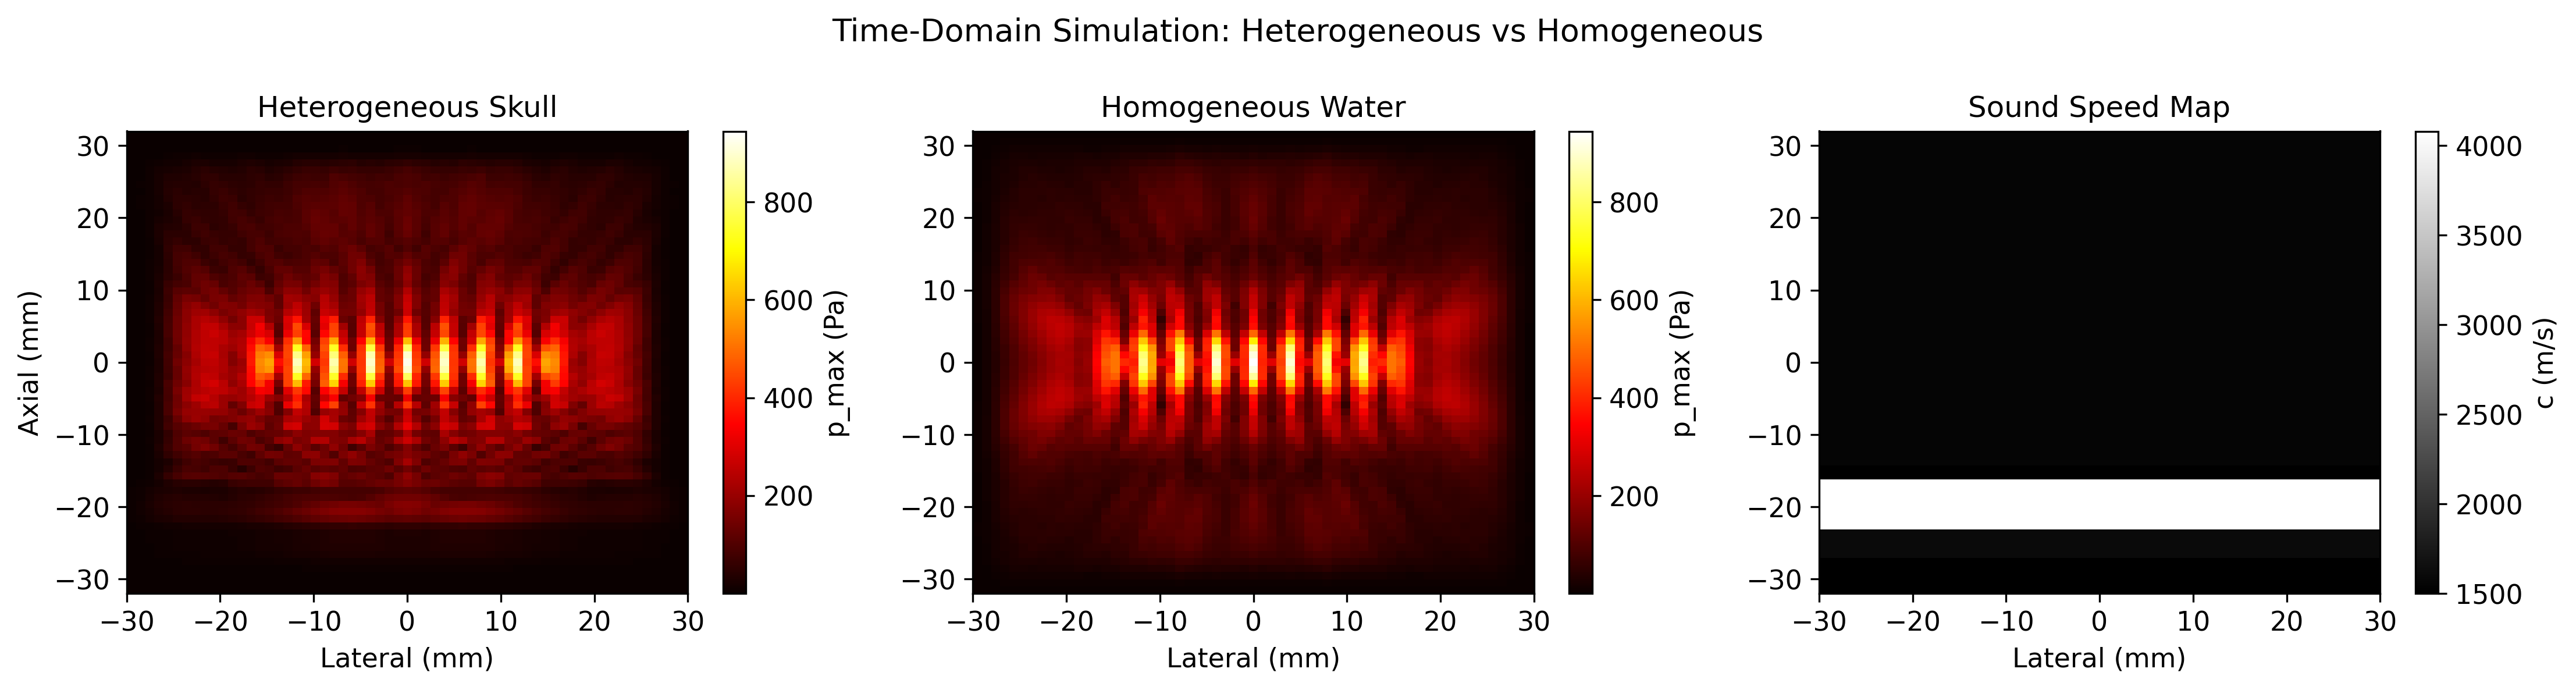
\includegraphics[width=\textwidth]{figures/fig4_het_vs_water.png}
  \caption{Time-domain simulation with a 64-element transducer through
    heterogeneous skull layers (left) vs.\ homogeneous water (center).
    Right: sound speed map showing the tissue layer structure.}
  \label{fig:het_vs_water}
\end{figure}

% ============================================================================
\section{Discussion}
\label{sec:discussion}
% ============================================================================

\subsection{Differentiable tFUS in the JAX neuroimaging stack}

The integration of j-Wave into OpenLIFU via JAX creates a differentiable
path from tissue segmentation to acoustic simulation. This enables:

\begin{enumerate}
  \item \textbf{Gradient-based phase correction}: Optimize transducer
    delays $\tau_i$ by backpropagating through the Helmholtz solver to
    maximize focal pressure, replacing the reciprocity-based approach
    that requires a separate simulation per target.
  \item \textbf{SBI for treatment planning}: Train neural density
    estimators on j-Wave simulations to perform amortized Bayesian
    inference over skull acoustic properties given measured focal
    pressure, enabling real-time treatment adaptation.
  \item \textbf{End-to-end multi-modal optimization}: With sbi4dwi
    providing tissue microstructure and NeuroJAX providing cortical
    dynamics, the entire path from diffusion MRI to neuromodulation
    target to acoustic simulation to treatment delivery is
    differentiable.
\end{enumerate}

\subsection{j-Wave extension opportunities}

During this work, we identified several gaps in j-Wave that would
benefit the broader community:

\begin{itemize}
  \item \textbf{Turnkey CW solver}: A high-level
    \texttt{simulate\_cw\_propagation(medium, f0, sources)} wrapping the
    raw Helmholtz operator.
  \item \textbf{Bowl/array source primitives}: The current
    \texttt{Sources} class only supports point sources; a
    \texttt{TransducerArray} class would simplify transcranial
    simulations.
  \item \textbf{Streaming max/min sensor}: Accumulating running
    max/min in the \texttt{jax.lax.scan} carry state would eliminate the
    memory bottleneck of storing the full pressure time series.
  \item \textbf{Sources.on\_grid clamping}: JAX's out-of-bounds index
    clamping causes the source to keep emitting at its last sample value
    after the signal ends, rather than zeroing out.
\end{itemize}

\subsection{SCI head model validation}

The SCI multi-modal head model provides co-registered T1w/T2w, diffusion
MRI, and tissue segmentation labels. By processing the tissue labels
through \texttt{HeterogeneousSkullSegmentation(source='labels')} and
feeding the acoustic property maps to the j-Wave Helmholtz solver, we
obtain patient-specific focal pressure predictions that can be validated
against hydrophone measurements or compared across the ITRUSST solver
ensemble. The shared JAX backend with sbi4dwi and NeuroJAX enables
joint optimization of neuromodulation targeting and acoustic delivery.

% ============================================================================
\section{Software}
\label{sec:software}
% ============================================================================

All code is open source under the MIT license:
\begin{itemize}
  \item \textbf{OpenLIFU}: \url{https://github.com/OpenwaterHealth/openlifu-python}
  \item \textbf{j-Wave}: \url{https://github.com/ucl-bug/jwave}
  \item \textbf{NeuroJAX}: \url{https://github.com/m9h/neurojax}
  \item \textbf{sbi4dwi}: \url{https://github.com/m9h/sbi4dwi}
\end{itemize}

Benchmark scripts and Modal deployment configurations are included in
the \texttt{benchmarks/} directory of the OpenLIFU repository.

% ============================================================================
\bibliography{references}
% ============================================================================

\end{document}
